\section*{سوال ۱}

مفهوم
\lr{AMI}
یا
\lr{Ambient Intelligence}
چیست و آینده آن به چه صورتی است؟

\section*{جواب سوال ۱}

\begin{figure}[H]
	\centering
	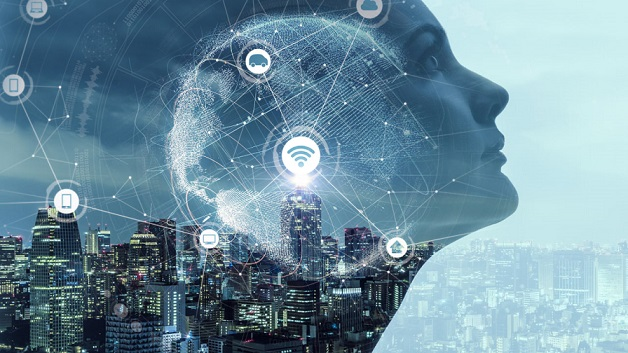
\includegraphics{pic1.jpg}
	\label{fig:label4}
\end{figure}

\lr{Ambient Intelligence (AMI)}
به عنوان یک مفهوم در اواخر دهه 1990 توسط مؤسسات تحقیقاتی اروپایی مطرح شد، به ویژه در پروژه‌های تحقیقاتی اتحادیه اروپا. ایده اصلی پشت AMI این است که فناوری‌های پیشرفته را در محیط‌های روزمره به گونه‌ای یکپارچه و نامرئی ادغام کنیم تا به طور هوشمند به نیازهای انسانی پاسخ دهند. این مفهوم بر اساس پیشرفت‌هایی در زمینه هوش مصنوعی، اینترنت اشیا (IoT) و شبکه‌های ارتباطی بنا نهاده شده است.
\section*{معرفی و تعریف}

\lr{Ambient Intelligence}
به یک محیط پویا و واکنشی اشاره دارد که در آن دستگاه‌ها و سیستم‌های مختلف به طور خودکار با یکدیگر و با کاربران خود ارتباط برقرار می‌کنند تا تجربه‌ای انطباق‌پذیر و هوشمند فراهم آورند. در چنین محیطی، دستگاه‌ها می‌توانند بدون دخالت مستقیم انسانی تصمیماتی بگیرند، که این امر به افزایش راحتی، بهره‌وری و ایمنی کمک می‌کند.


\begin{figure}[H]
	\centering
	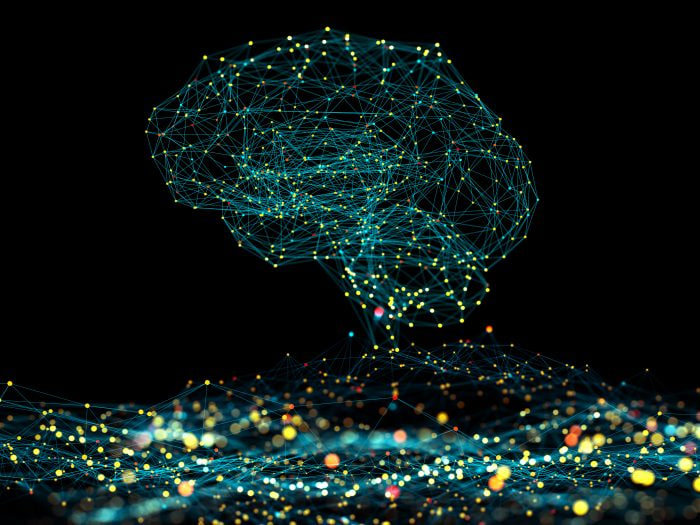
\includegraphics{pic2.jpg}
	\label{fig:label4}
\end{figure}

\section*{حال حاضر و آینده AMI}
در حال حاضر،
\lr{AMI}
در حال پیدا کردن جایگاهی است در بسیاری از جنبه‌های زندگی مدرن، از خانه‌های هوشمند گرفته تا محیط‌های کاری و حتی شهرهای هوشمند. با گسترش اینترنت اشیاء 
\lr{(IoT)}
و فناوری‌های مانند هوش مصنوعی و یادگیری ماشین، این سیستم‌ها به طور فزاینده‌ای می‌توانند اقدامات و نیازهای انسانی را پیش‌بینی کنند و به آنها پاسخ دهند.

آینده‌ی
\lr{AMI}
می‌تواند شامل پیشرفت‌های چشمگیری باشد، از جمله:
\begin{itemize}
	\item انطباق‌پذیری بیشتر: محیط‌ها به طور فعال با نیازها و ترجیحات افراد سازگار خواهند شد.
	\item پیشرفت‌های در حوزه حریم خصوصی و امنیت: با افزایش نگرانی‌های مربوط به داده‌های شخصی، فناوری‌های جدید باید به گونه‌ای طراحی شوند که حفظ حریم خصوصی را تضمین کنند.
	\item همگرایی بیشتر با پوشیدنی‌ها: دستگاه‌های پوشیدنی همچنان با محیط اطراف ادغام خواهند شد، اجازه دادن به کاربران برای انجام تعاملات پیچیده تر با محیط.
	\item استقلال و خودمختاری: سیستم‌های \lr{AMI} ممکن است قادر به انجام تصمیم‌گیری‌های پیچیده‌تر بدون نیاز به دخالت انسانی باشند.
	\item تعاملات انسان-ماشین طبیعی‌تر: با پیشرفت در زمینه شناسایی گفتار و پردازش زبان طبیعی، تعامل با سیستم‌های \lr{AMI} بیش از پیش طبیعی و انسانی خواهد شد.
\end{itemize}
این فناوری‌ها نه تنها زندگی روزمره را آسان‌تر می‌کنند، بلکه می‌توانند برای کمک به افراد معلول، سالمندان و دیگر گروه‌های آسیب‌پذیر در جامعه به کار روند.

\section*{سیستم‌های نهفته در \lr{AMI}}

مفهوم
\textbf{\lr{Ambient Intelligence (AMI)}}
با سیستم‌های نهفته
(\textbf{\lr{Embedded Systems}})
در ارتباط تنگاتنگی قرار دارد. سیستم‌های نهفته رایانه‌های تخصصی هستند که در دستگاه‌های الکترونیکی برای انجام وظایف خاص طراحی شده‌اند. این سیستم‌ها اغلب در برنامه‌هایی که نیاز به پردازش داده‌های محلی، پاسخ‌گویی سریع و ادغام با دنیای فیزیکی دارند، به کار برده می‌شوند. در \lr{AMI} ، سیستم‌های نهفته نقش محوری دارند چرا که به این سیستم‌ها اجازه می‌دهند تا به صورت همه‌جانبه، در محیط‌های فیزیکی ادغام شوند و تجربه‌های کاربری غنی و هوشمندانه‌ای ارائه دهند.

\subsection*{تعامل با محیط}
سیستم‌های نهفته در \lr{AMI} می‌توانند از طریق سنسورها و اکچویتورها با محیط اطراف خود تعامل داشته باشند. سنسورها داده‌هایی از محیط جمع‌آوری می‌کنند، مانند دما، رطوبت، نور، حرکت، و صدا. سپس این داده‌ها توسط پردازنده‌های سیستم‌های نهفته تحلیل و پردازش می‌شوند تا اطلاعاتی مفید برای اتخاذ تصمیم‌های هوشمندانه فراهم آورند.

\subsection*{خودکارسازی و پاسخگویی}
سیستم‌های نهفته می‌توانند فعالیت‌های خودکاری مانند کنترل دما، روشنایی، و سیستم‌های امنیتی را اجرا کنند. به عنوان مثال، در یک خانه هوشمند، سیستم‌های نهفته ممکن است تشخیص دهند که هیچ کس در اتاق حضور ندارد و به صورت خودکار چراغ‌ها را خاموش کنند تا انرژی صرفه‌جویی شود.

\subsection*{هوش مصنوعی و یادگیری ماشین}
برای رسیدن به سطح بالایی از هوشمندی، سیستم‌های نهفته در \lr{AMI} اغلب با الگوریتم‌های یادگیری ماشین و هوش مصنوعی تجهیز می‌شوند. این الگوریتم‌ها به سیستم‌ها امکان می‌دهند تا از تجربیات گذشته یاد بگیرند، الگوهای رفتاری را شناسایی کنند، و پیش‌بینی‌هایی در مورد نیازهای آینده کاربران داشته باشند.

\subsection*{امنیت و حریم خصوصی}
یکی از چالش‌های اصلی سیستم‌های نهفته در \lr{AMI} حفاظت از اطلاعات شخصی و حفظ حریم خصوصی کاربران است. با توجه به میزان داده‌های حساسی که جمع‌آوری و پردازش می‌شود، لازم است سیستم‌های امنیتی و رمزنگاری پیشرفته‌ای برای محافظت از این اطلاعات در برابر دسترسی‌های غیرمجاز ادغام شوند.

\subsection*{بهینه‌سازی مصرف انرژی}
سیستم‌های نهفته باید بتوانند با مصرف کم انرژی کار کنند تا به توسعه پایدار کمک کنند. در \lr{AMI}، این مسئله به معنای طراحی سخت‌افزار و نرم‌افزارهایی است که کارآمدی انرژی را به حداکثر برسانند و در عین حال کارایی بالایی داشته باشند.

در نهایت، سیستم‌های نهفته به عنوان مغز و مرکز کنترل در مفهوم \textbf{\lr{Ambient Intelligence}} عمل می‌کنند، که به آن‌ها اجازه می‌دهد تا به صورت همزمان هم هوشمند و هم پنهان باقی بمانند. این امر موجب می‌شود تا تجربه‌های کاربری به شکلی طبیعی و بی‌درز با زندگی روزمره ادغام شوند.
